\documentclass{article}
\usepackage{listings}
\usepackage{graphicx}
\title{Operational Statistics for SAR Image Report}
\author{Jinkai Cheng, School of Artificial Intelligence}
\date\today
\begin{document}
\maketitle
\section{load required files and packages}
\begin{lstlisting}[frame=tb]
source("myread.ENVI.R")
source("imagematrix.R")
require(ggplot2)
require(reshape2)
require(ggthemes)
require(maxLik)
\end{lstlisting}

\section{sample forest region from image}
\begin{lstlisting}[frame=tb]
imagepath <- "../Statistics-SAR-Intensity-master/Data/Images/ESAR/"
HH_Complex <- myread.ENVI(paste(imagepath, "ESAR97HH.DAT", sep = ""),
paste(imagepath, "ESAR97HH.hdr", sep = ""))
HH_Intensity <- (Mod(HH_Complex))^2
example <- HH_Intensity[1300:1400,2280:2480]
vec_example <- data.frame(HH=as.vector(example))
plot(imagematrix(equalize(example)))
imagematrixPNG(name = "./forest.png", imagematrix(equalize(example)))
vec_example <- data.frame(HH=as.vector(example))
summary(vec_example)

       HH           
Min.   :     0.91  
1st Qu.:  2743.85  
Median :  6678.06  
Mean   : 10278.44  
3rd Qu.: 13632.24  
Max.   :276306.28 
\end{lstlisting}

\begin{figure}[htb]
	\centering
	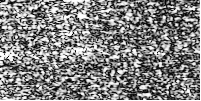
\includegraphics[width=0.5\linewidth]{forest.png}
	\caption{Forest Region}
	\label{fig:forest}
\end{figure}



\section{Histogram}
\begin{lstlisting}[frame=tb]
binwidth_complete <- 2*IQR(vec_example$HH)*length(vec_example$HH)^(-1/3)
ggplot(data=vec_example, aes(x=HH)) + 
geom_histogram(aes(y=..density..), 
binwidth = binwidth_complete) + 
xlab("Intensities") +
ylab("Proportions") +
ggtitle("Complete Histogram") +
theme_few()
ggsave(filename = "./HistogramExample.pdf")
\end{lstlisting}

\begin{figure}
	\centering
	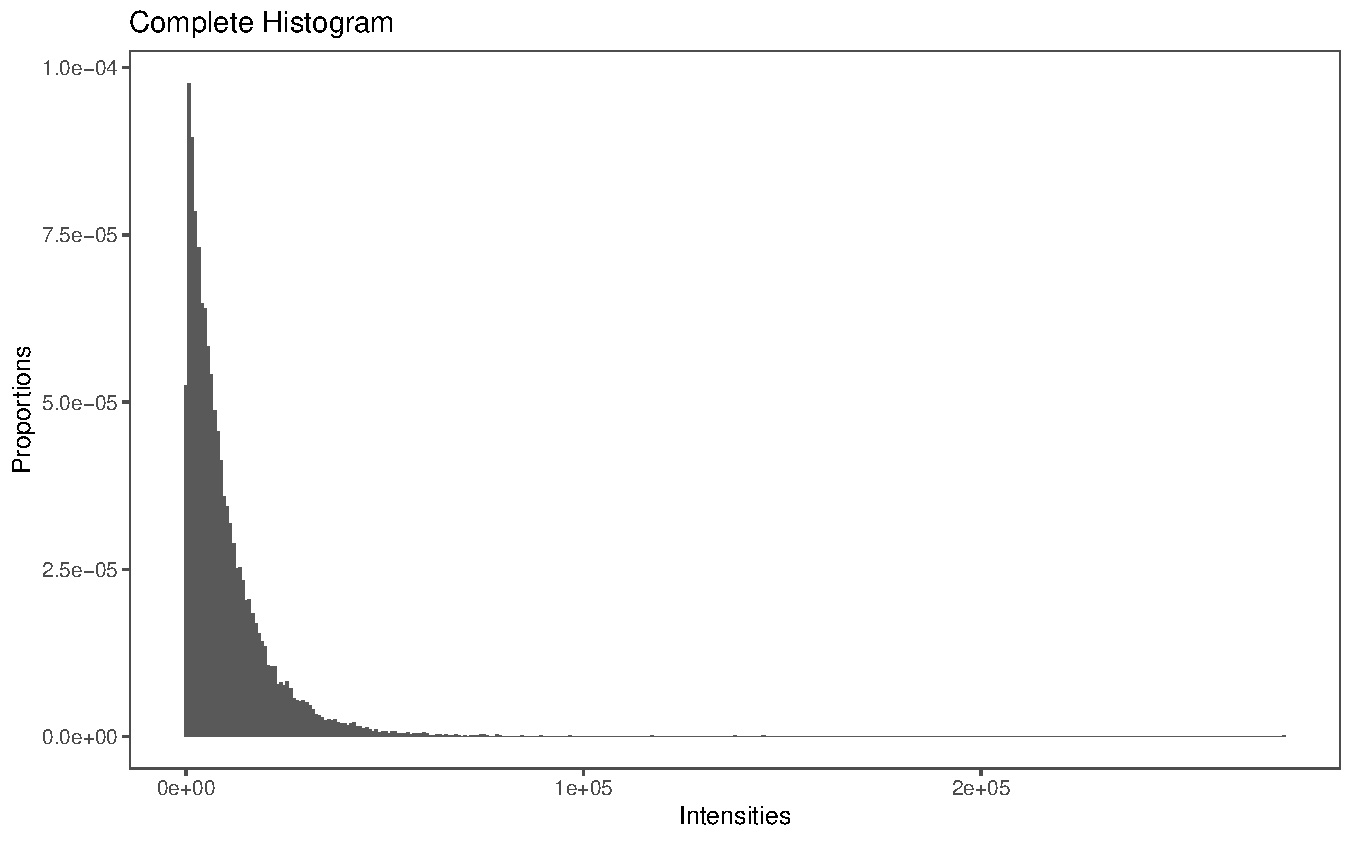
\includegraphics[width=0.5\linewidth]{HistogramExample.pdf}
	\caption{HistogramExample}
	\label{fig:HistogramExample}
\end{figure}

\section{LogLikelihood}
\begin{lstlisting}[frame=tb]
LogLikelihoodLknown <- function(params) {

p_alpha <- -abs(params[1])
p_gamma <- abs(params[2])
p_L <- abs(params[3])

n <- length(z)

return(
n*(lgamma(p_L-p_alpha) - p_alpha*log(p_gamma) - lgamma(-p_alpha)) + 
(p_alpha-p_L)*sum(log(p_gamma + z*p_L)) 
)
}
\end{lstlisting}
\section{Estimation}
\begin{lstlisting}[frame=tb]
z <- vec_example$HH

estim.exampleML <- maxNR(LogLikelihoodLknown, 
start=c(estim.example$alpha, estim.example$gamma,1), 
activePar=c(TRUE,TRUE,FALSE))$estimate[1:2]
> estim.exampleML
[1]    -3.141452 23517.332553
\end{lstlisting}
results all above
\end{document}
